\chapter{हमारे चारों ओर ध्वनि}\label{ch:g3:sound-around-us}

अपना पसंदीदा गीत गुनगुनाओ --- और गुनगुनाते समय दो उँगलियाँ हल्के से
अपने गले के सामने रखो। वह थरथराहट महसूस हुई? तुमने अभी-अभी किसी \omterm{def:g3:sound-around-us:sound}{ध्वनि}
को उसके जन्मस्थान पर छू लिया। हर आवाज़, हर ढोल, हर चरमराता दरवाज़ा
अपनी \omterm{def:g3:sound-around-us:sound}{ध्वनि} ठीक इसी तरह बनाता है, और यह अध्याय उसी तरकीब का शिकार करने
निकला है।

\section{ध्वनियाँ जन्म कहाँ लेती हैं}

\begin{definition}[कंपन]\label{def:g3:sound-around-us:vibration}
\emph{कंपन}\index{कंपन} बहुत तेज़ थरथराहट है --- आगे-पीछे होती वह
हरकत जो हर सेकंड कई बार दोहराई जाती है, और अकसर इतनी तेज़ होती है कि
आँख उसका पीछा नहीं कर पाती। छेड़ी हुई गिटार की तार कंपन करती है:
तुम्हें बस एक धुँधलापन दिखता है, पर उँगली की नोक को उसकी भनभनाहट
महसूस होती है।
\end{definition}

\begin{definition}[ध्वनि]\label{def:g3:sound-around-us:sound}
\emph{ध्वनि}\index{ध्वनि} वह है जो हम तब सुनते हैं जब कोई चीज़ \omterm{def:g3:sound-around-us:vibration}{कंपन}
करती है और उसकी थरथराहट \omterm{def:g2:air-around-us:air}{हवा} में से होकर हमारे कानों तक पहुँचती है।
\omterm{def:g3:sound-around-us:vibration}{कंपन} करने वाली चीज़ उस ध्वनि का \emph{स्रोत} है --- कोई तार, ढोल की
खाल, कोई घंटी, या तुम्हारा अपना गला।
\end{definition}

\begin{method}[चावल को नचाना]\label{met:g3:sound-around-us:rice}
\omterm{def:g3:sound-around-us:sound}{ध्वनि} को जन्म लेते \emph{देखने} के लिए:
\begin{enumerate}
  \item ढोल की खाल पर (या डिब्बे के प्लास्टिक ढक्कन पर, या तने हुए
        गुब्बारे की झिल्ली पर) चावल के कुछ दाने बिखेरो;
  \item दानों के पास खाल पर थाप दो --- धम: दाने उछल पड़ते हैं!
  \item अब बिलकुल पास से खाल पर सिर्फ़ \emph{चिल्लाओ}: दाने फिर
        थरथराते हैं, बिना छुए ही।
\end{enumerate}
खाल जब भी बजती है तब \omterm{def:g3:sound-around-us:vibration}{कंपन} करती है --- और तुम्हारे मुँह से आई \omterm{def:g3:sound-around-us:sound}{ध्वनि} भी
उसे थरथरा देती है।
\end{method}

\begin{omfigure}
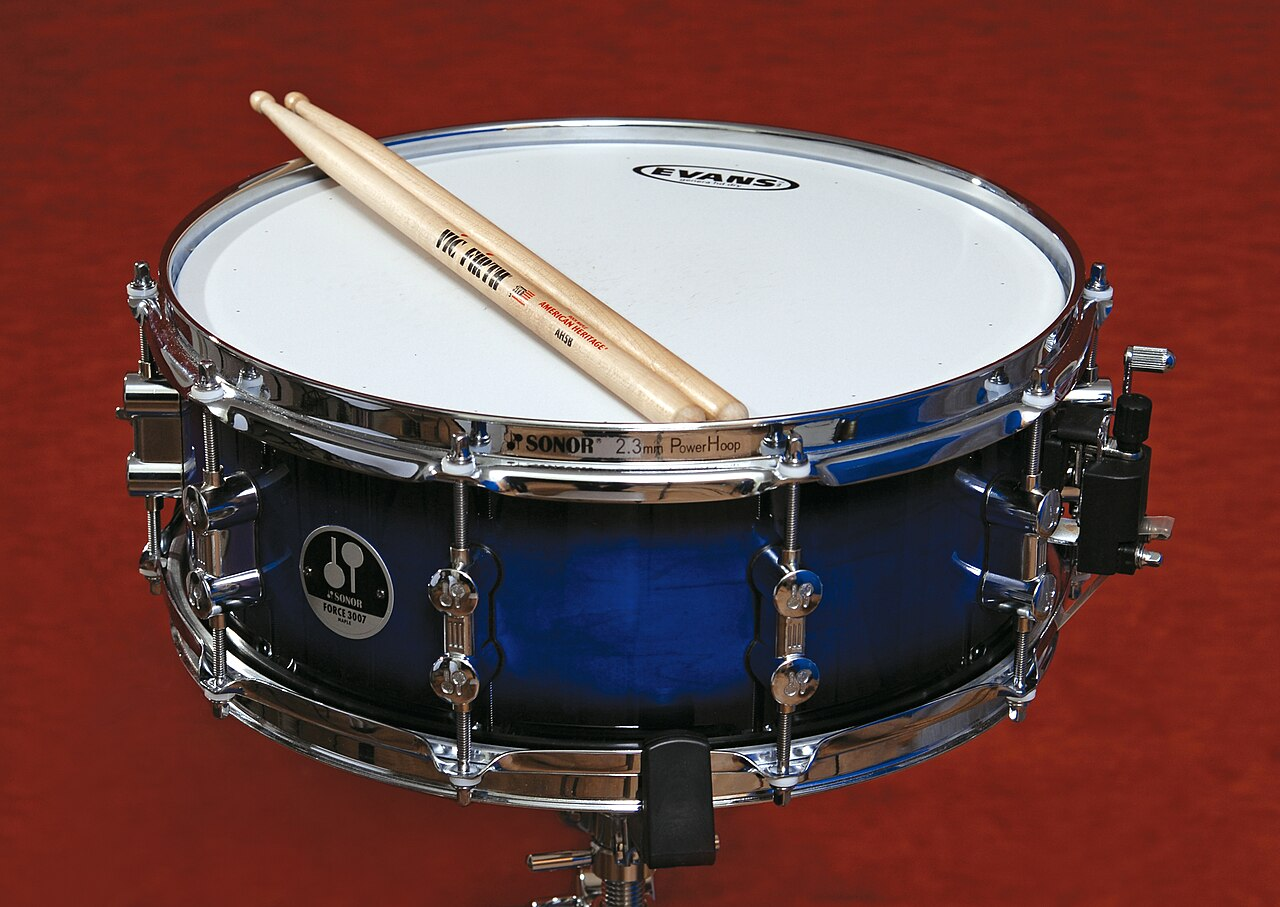
\includegraphics[width=0.58\linewidth]{images/book1/drum.jpg}

{\small चावल वाले प्रयोग के लिए असली ढोल: सफ़ेद खाल ही थरथराने वाला
हिस्सा है। उस पर कुछ दाने बिखेरो, उनके पास थाप दो --- बजती हुई खाल
थरथराती खाल है, और चावल नाचकर इसे साबित कर देता है।
\emph{चित्र: व्लादीमिर मोरोज़ोव, CC BY 2.0.}}
\end{omfigure}

\begin{proposition}[कंपन नहीं, तो ध्वनि नहीं]\label{prop:g3:sound-around-us:novib}
हर \omterm{def:g3:sound-around-us:sound}{ध्वनि} किसी \omterm{def:g3:sound-around-us:vibration}{कंपन} से आती है --- और \omterm{def:g3:sound-around-us:vibration}{कंपन} रुकते ही \omterm{def:g3:sound-around-us:sound}{ध्वनि} भी उसी पल रुक
जाती है। झाँझ पर चोट मारो और उसे गूँजने दो; फिर उसे दोनों हाथों से
कसकर पकड़ लो: तुम्हारी पकड़ जिस पल थरथराहट रोकती है, उसी पल सन्नाटा।
\end{proposition}

\begin{example}[हर जगह ध्वनि के स्रोत]\label{ex:g3:sound-around-us:sources}
हर \omterm{def:g3:sound-around-us:sound}{ध्वनि} के पीछे का \omterm{def:g3:sound-around-us:vibration}{कंपन} ढूँढ़ो: गिटार --- छेड़ी हुई तारें थरथराती
हैं; ढोल --- चोट खाई खाल थरथराती है; तुम्हारी आवाज़ --- फेफड़ों की
\omterm{def:g2:air-around-us:air}{हवा} तेज़ी से निकलते समय गले की दो नन्ही झिल्लियाँ थरथराती हैं (यही वह
भनभनाहट है जो तुम्हारी उँगलियों ने महसूस की); भनभनाती मक्खी ---
उसके पंख हर सेकंड सैकड़ों बार थरथराते हैं; ज़ोर से बंद किया दरवाज़ा
--- पूरा दरवाज़ा और उसकी चौखट पल भर के लिए काँप उठते हैं।
\end{example}

\section{तेज़ और धीमी, ऊँची और नीची}

\begin{example}[तेज़ ध्वनि यानी बड़ा कंपन]\label{ex:g3:sound-around-us:loud}
तने हुए रबर बैंड को हल्के-से छेड़ो: छोटा-सा धुँधलापन, धीमी टनक। उसे
ज़ोर से छेड़ो: चौड़ा धुँधलापन, तेज़ टनक। स्रोत जितने ज़ोर से थरथराता
है --- यानी उसका आगे-पीछे होना जितना चौड़ा होता है --- \omterm{def:g3:sound-around-us:sound}{ध्वनि} उतनी ही
\emph{तेज़} होती है। चावल के दानों को भी देखो: हल्की थाप उन्हें
सिहरा देती है, ज़ोरदार धमाका उन्हें \omterm{def:g2:air-around-us:air}{हवा} में उछाल देता है।
\end{example}

\begin{example}[ऊँची और नीची]\label{ex:g3:sound-around-us:pitch}
खुले डिब्बे पर एक रबर बैंड तानकर छेड़ो; फिर उसे बीच में दबाकर पकड़ो
और छोटे आधे हिस्से को छेड़ो: टनक \emph{ऊँची} हो जाती है, चिड़िया की
चहचहाहट जैसी। छोटी, कसी और पतली चीज़ें ज़्यादा तेज़ी से थरथराती हैं
और ऊँचा गाती हैं; लंबी, ढीली और मोटी चीज़ें धीरे थरथराती हैं और नीचा
गाती हैं। इसीलिए नन्ही बाँसुरी चहकती है और बड़ा तुरही-भोंपू गुर्राता
है --- और इसीलिए गिटार की सबसे पतली तार सबसे ऊँचा गाती है।
\end{example}

\begin{omfigure}
\begin{tikzpicture}[scale=0.85]
  % whole band, stretched over the open box, vibrating end to end
  \draw[thick] (0.3,0) rectangle (4.9,1.1);
  \draw[omDef, very thick] (0.3,1.1) -- (4.9,1.1);
  \draw[dashed, omDef] (0.3,1.1) .. controls (2.6,1.62) .. (4.9,1.1);
  \draw[dashed, omDef] (0.3,1.1) .. controls (2.6,0.58) .. (4.9,1.1);
  \node[below, font=\small, align=center] at (2.6,-0.3)
    {पूरा बैंड:\\धीमा कंपन, नीची टनक};
  % pinched at the middle: only the short half vibrates
  \draw[thick] (6.5,0) rectangle (11.1,1.1);
  \draw[omDef, very thick] (6.5,1.1) -- (11.1,1.1);
  \fill[omExo] (8.8,1.1) circle (0.1);
  \node[above, font=\footnotesize, omExo] at (8.8,1.32) {पकड़};
  \draw[dashed, omDef] (8.8,1.1) .. controls (9.95,1.45) .. (11.1,1.1);
  \draw[dashed, omDef] (8.8,1.1) .. controls (9.95,0.75) .. (11.1,1.1);
  \node[below, font=\small, align=center] at (8.8,-0.3)
    {दबाकर छोटा किया:\\तेज़ कंपन, ऊँची टनक};
\end{tikzpicture}

{\small रबर बैंड वाला गिटार: पूरा बैंड अपने दोनों सिरों पर बँधा रहकर
बीच में सबसे चौड़ा झूलता है और नीचा गाता है; दबाकर छोटा किया गया आधा
हिस्सा ज़्यादा तेज़ी से थरथराता है और ऊँचा गाता है।}
\end{omfigure}

\begin{remark}[कान के भीतर के नन्हे ढोल को बचाओ]\label{rem:g3:sound-around-us:ears}
तुम्हारे कान की गहराई में काग़ज़ से भी पतली एक नन्ही झिल्ली हर आती
हुई \omterm{def:g3:sound-around-us:sound}{ध्वनि} के साथ थरथराती है, ठीक चावल वाले ढोल की तरह। बहुत तेज़
ध्वनियाँ उसे बहुत ज़ोर से हिला देती हैं: बहुत तेज़ संगीत, मशीनें और
पटाख़े उसे हमेशा के लिए बिगाड़ सकते हैं, और वह दोबारा नहीं बनती। तेज़
शोर के पास कान ढक लो, और किसी के कान में कभी मत चिल्लाओ --- कानों की
पलकें नहीं होतीं।
\end{remark}

\section{स्रोत से कान तक}

\begin{example}[एक ताली की यात्रा]\label{ex:g3:sound-around-us:journey}
मैदान के उस पार कोई साथी ताली बजाता है। ताली \omterm{def:g2:air-around-us:air}{हवा} को थरथरा देती है;
वह थरथराहट \omterm{def:g2:air-around-us:air}{हवा} में हर दिशा में फैलती है, ठीक वैसे जैसे तालाब में गिरे
कंकड़ के चारों ओर छल्ले; उसका कुछ हिस्सा तुम्हारे कान तक पहुँचता है
और कान की नन्ही झिल्ली को थरथरा देता है --- और तुम्हें ताली सुनाई देती
है। स्रोत, यात्रा, कान: आज तक तुमने जो भी \omterm{def:g3:sound-around-us:sound}{ध्वनि} सुनी है उसने यही सफ़र
किया है। यह सफ़र कितना तेज़ होता है, और किन-किन चीज़ों में से गुज़र
सकता है? अगले साल का \omterm{def:g3:sound-around-us:sound}{ध्वनि} वाला अध्याय ठीक यही सवाल उठाता है।
\end{example}

\section{अभ्यास}

\begin{exercise}[$\star$]\label{exo:g3:sound-around-us:1}
\omterm{def:g3:sound-around-us:vibration}{कंपन} क्या है? इनमें \omterm{def:g3:sound-around-us:vibration}{कंपन} करने वाला हिस्सा बताओ: गिटार; \ ढोल; \
तुम्हारी आवाज़; \ भनभनाती मक्खी।
\end{exercise}

\begin{exercise}[$\star$]\label{exo:g3:sound-around-us:2}
चावल वाले प्रयोग में उछलते दाने बजती हुई ढोल की खाल के बारे में क्या
साबित करते हैं?
\end{exercise}

\begin{exercise}[$\star$]\label{exo:g3:sound-around-us:3}
गूँजती हुई झाँझ पकड़ते ही वह चुप क्यों हो जाती है? यहाँ अध्याय का
कौन-सा नियम काम कर रहा है?
\end{exercise}

\begin{exercise}[$\star$]\label{exo:g3:sound-around-us:4}
रबर बैंड की टनक \emph{तेज़} करनी हो तो अपनी छेड़ में क्या बदलोगे? तब
बैंड का धुँधलापन कैसा दिखता है?
\end{exercise}

\begin{exercise}[$\star$]\label{exo:g3:sound-around-us:5}
कौन ऊँचा गाता है: दबाकर छोटा किया बैंड या पूरा बैंड? \ नन्ही
बाँसुरी या बड़ा तुरही-भोंपू? \ गिटार की सबसे पतली तार या सबसे मोटी?
\end{exercise}

\begin{exercise}[$\star$]\label{exo:g3:sound-around-us:6}
गले पर उँगलियाँ रखकर गुनगुनाओ, फिर गुनगुनाना बंद कर दो। तुम्हारी
उँगलियों को क्या महसूस होता है, और वह ठीक कब बंद हो जाता है?
\end{exercise}

\begin{exercise}[$\star$]\label{exo:g3:sound-around-us:7}
तुम्हारे साथी के हाथों से तुम्हारे कान तक ताली की यात्रा तीन क़दमों
में सुनाओ।
\end{exercise}

\begin{exercise}[$\star$]\label{exo:g3:sound-around-us:8}
बहुत तेज़ ध्वनियों को कानों से दूर क्यों रखना चाहिए? कान के भीतर की
कौन-सी नन्ही चीज़ ख़तरे में रहती है, और इस अध्याय की किस चीज़ से वह
मिलती-जुलती है?
\end{exercise}

\begin{exercise}[$\star$]\label{exo:g3:sound-around-us:9}
किसी बाजे की कंघी में अलग-अलग लंबाई के दाँते होते हैं। ऊँचे सुर
कौन-से दाँते बजाते हैं और नीचे कौन-से?
\cref{ex:g3:sound-around-us:pitch} के नियम से उत्तर दो।
\end{exercise}

\begin{exercise}[$\star\star$]\label{exo:g3:sound-around-us:10}
काँच की बोतल में पानी भरो और उसके मुँह पर तिरछी फूँक मारो: एक हूक!
और पानी डालो और फिर फूँक मारो: हूक ऊँची हो जाती है। हूक बनाने के लिए
थरथरा क्या रहा है --- काँच, पानी, या भीतर की \omterm{def:g2:air-around-us:air}{हवा}? ``छोटा ऊँचा गाता
है'' वाले नियम से अपने उत्तर के पक्ष में तर्क दो।
\end{exercise}

\begin{exercise}[$\star\star$]\label{exo:g3:sound-around-us:11}
माया कहती है: ``टेलीविज़न की आवाज़ बंद हो तब भी परदा हिलता रहता है
--- यानी अकेली हरकत ही \omterm{def:g3:sound-around-us:sound}{ध्वनि} बना देती होगी।''
\cref{def:g3:sound-around-us:sound} और चावल वाले प्रयोग से समझाओ कि
\omterm{def:g3:sound-around-us:sound}{ध्वनि} किस तरह की हरकत से बनती है, और परदे के चित्र कोई \omterm{def:g3:sound-around-us:sound}{ध्वनि} क्यों
नहीं बनाते।
\end{exercise}
